\documentclass[journal]{vgtc}                % final (journal style)
%\documentclass[review,journal]{vgtc}         % review (journal style)
%\documentclass[widereview]{vgtc}             % wide-spaced review
%\documentclass[preprint,journal]{vgtc}       % preprint (journal style)

%% Uncomment one of the lines above depending on where your paper is
%% in the conference process. ``review'' and ``widereview'' are for review
%% submission, ``preprint'' is for pre-publication, and the final version
%% doesn't use a specific qualifier.

%% Please use one of the ``review'' options in combination with the
%% assigned online id (see below) ONLY if your paper uses a double blind
%% review process. Some conferences, like IEEE Vis and InfoVis, have NOT
%% in the past.

%% Please note that the use of figures other than the optional teaser is not permitted on the first page
%% of the journal version.  Figures should begin on the second page and be
%% in CMYK or Grey scale format, otherwise, colour shifting may occur
%% during the printing process.  Papers submitted with figures other than the optional teaser on the
%% first page will be refused. Also, the teaser figure should only have the
%% width of the abstract as the template enforces it.

%% These few lines make a distinction between latex and pdflatex calls and they
%% bring in essential packages for graphics and font handling.
%% Note that due to the \DeclareGraphicsExtensions{} call it is no longer necessary
%% to provide the the path and extension of a graphics file:
%% 
\includegraphics{diamondrule} is completely sufficient.
%%
\ifpdf%                                % if we use pdflatex
  \pdfoutput=1\relax                   % create PDFs from pdfLaTeX
  \pdfcompresslevel=9                  % PDF Compression
  \pdfoptionpdfminorversion=7          % create PDF 1.7
  \ExecuteOptions{pdftex}
  \usepackage{graphicx}                % allow us to embed graphics files
  \DeclareGraphicsExtensions{.pdf,.png,.jpg,.jpeg} % for pdflatex we expect .pdf, .png, or .jpg files
\else%                                 % else we use pure latex
  \ExecuteOptions{dvips}
  \usepackage{graphicx}                % allow us to embed graphics files
  \DeclareGraphicsExtensions{.eps}     % for pure latex we expect eps files
\fi%

%% it is recomended to use ``\autoref{sec:bla}'' instead of ``Fig.~\ref{sec:bla}''
\graphicspath{{figures/}{pictures/}{images/}{./}} % where to search for the images

\usepackage{microtype}                 % use micro-typography (slightly more compact, better to read)
\PassOptionsToPackage{warn}{textcomp}  % to address font issues with \textrightarrow
\usepackage{textcomp}                  % use better special symbols
\usepackage{mathptmx}                  % use matching math font
\usepackage{times}                     % we use Times as the main font
\renewcommand*\ttdefault{txtt}         % a nicer typewriter font
\usepackage{cite}                      % needed to automatically sort the references
\usepackage{tabu}                      % only used for the table example
\usepackage{booktabs}                  % only used for the table example
%% We encourage the use of mathptmx for consistent usage of times font
%% throughout the proceedings. However, if you encounter conflicts
%% with other math-related packages, you may want to disable it.

%% In preprint mode you may define your own headline.
%\preprinttext{To appear in IEEE Transactions on Visualization and Computer Graphics.}

%% If you are submitting a paper to a conference for review with a double
%% blind reviewing process, please replace the value ``0'' below with your
%% OnlineID. Otherwise, you may safely leave it at ``0''.
\onlineid{0}

%% declare the category of your paper, only shown in review mode
\vgtccategory{Research}
%% please declare the paper type of your paper to help reviewers, only shown in review mode
%% choices:
%% * algorithm/technique
%% * application/design study
%% * evaluation
%% * system
%% * theory/model
\vgtcpapertype{please specify}

%% Paper title.
\title{Visualization of Reported UFO Sightings}

%% This is how authors are specified in the journal style

%% indicate IEEE Member or Student Member in form indicated below
\author{Peter Bernstein, Emily Dutile, Abigail Skelton, and Lydia Zakynthinou}
\authorfooter{
%% insert punctuation at end of each item
\item
Emily Dutile and Abigail Skelton are graduate students at Northeastern University. E-mail: \{dutile.e, skelton.a\}@husky.neu.edu.
\item
Peter Bernstein and Lydia Zakynthinou are PhD students at Northeastern University. E-mail: \{bernstein.p, zakynthinou.l\}@husky.neu.edu.
}


%other entries to be set up for journal
\shortauthortitle{Biv \MakeLowercase{\textit{et al.}}: Visualization of Reported UFO Sightings}
%\shortauthortitle{Firstauthor \MakeLowercase{\textit{et al.}}: Paper Title}

%% Abstract section.
\abstract{Reports of unidentified flying objects (\textit{UFOs}) have sparked amateur research, government investigations,
 and large popular interest in the last five decades. Most reported UFOs are later identified as natural phenomena or
 conventional objects. However, there is a considerable body of reports about objects that are not identified, which are 
 often rumored as claims of observations of
 extraterrestrial crafts, raising questions about life on other planets and
 extraterrestrials visiting Earth. Scientists in their majority have naturally greeted the topic with
 skepticism but it widely recognized that answering these questions would be of great
 importance and a step towards understanding the universe. We provide an interactive
 visualization of the reported UFO sightings in the United States in the period of 1910-2014,
 aiming to help any interested user explore these sightings.
} % end of abstract

%% Keywords that describe your work. Will show as 'Index Terms' in journal
%% please capitalize first letter and insert punctuation after last keyword
\keywords{Visualization, Map, Interactivity, Unidentified Flying Object, UFO, United States.}

%% ACM Computing Classification System (CCS). 
%% See <http://www.acm.org/class/1998/> for details.
%% The ``\CCScat'' command takes four arguments.

\CCScatlist{ % not used in journal version
 \CCScat{K.6.1}{Management of Computing and Information Systems}%
{Project and People Management}{Life Cycle};
 \CCScat{K.7.m}{The Computing Profession}{Miscellaneous}{Ethics}
}

%% Uncomment below to include a teaser figure.
\teaser{
  \centering
  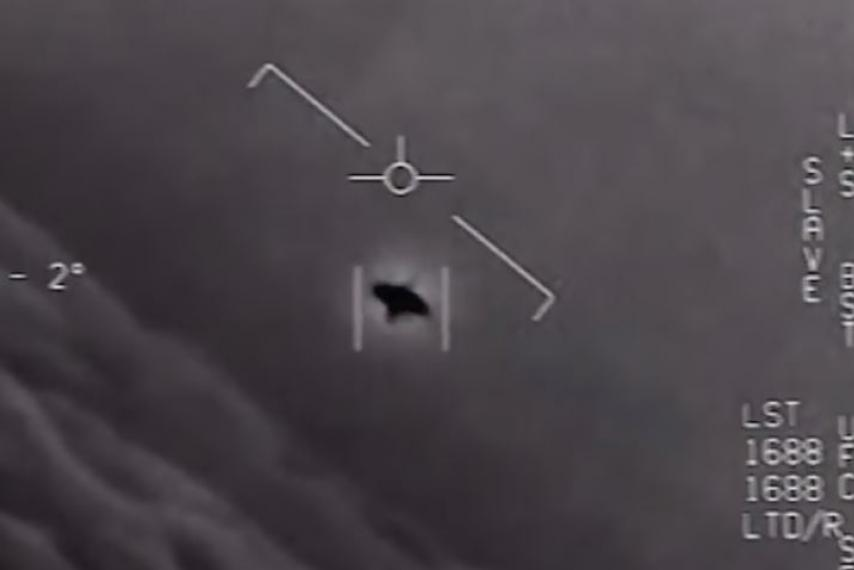
\includegraphics[width=\linewidth]{ufoimage}
  \caption{UFOs are ``proved beyond reasonable doubt": A rotating ``glowing aura" traveling at high speeds that was captured from a Navy F/A-18 Super Hornet. \cite{pentagon}}
	\label{fig:teaser}
}

%% Uncomment below to disable the manuscript note
\renewcommand{\manuscriptnotetxt}{}

%% Copyright space is enabled by default as required by guidelines.
%% It is disabled by the 'review' option or via the following command:
%\nocopyrightspace

\vgtcinsertpkg

%%%%%%%%%%%%%%%%%%%%%%%%%%%%%%%%%%%%%%%%%%%%%%%%%%%%%%%%%%%%%%%%
%%%%%%%%%%%%%%%%%%%%%% START OF THE PAPER %%%%%%%%%%%%%%%%%%%%%%
%%%%%%%%%%%%%%%%%%%%%%%%%%%%%%%%%%%%%%%%%%%%%%%%%%%%%%%%%%%%%%%%%

\begin{document}

%% The ``\maketitle'' command must be the first command after the
%% ``\begin{document}'' command. It prepares and prints the title block.

%% the only exception to this rule is the \firstsection command
\firstsection{Introduction}

\maketitle

%% \section{Introduction} %for journal use above \firstsection{..} instead
An unidentified flying object (UFO) is a perceived object in the sky that is not readily identified. The term UFO (initially, \textit{UFOB}) appeared in 1953 when the United States Air Force used it to describe ``any airborne object which by performance, aerodynamic characteristics, or unusual features, does not conform to any presently known aircraft or missile type, or which cannot be positively identified as a familiar object" \cite{ufowiki}. Since the 1950s, UFOs have become a major subject of interest in popular culture and an inspiration for several movies and books \cite{history}. Pop culture has glorified the idea of UFO's, specifically for their link to extraterrestrial life visiting earth.\\
\indent Although UFOs are largely connected to this theme, it is true that for most of the reported cases the objects are identified to be ordinary or to be caused by natural phenomena after careful investigation. Most commonly, UFOs are identified to actually be astronomical objects, aircrafts, balloons (e.g. weather, research balloons), atmospheric or light phenomena (e.g. clouds, mirages), other atmospheric objects (e.g. birds), or, in some rare cases, hoaxes. The percentage of reports of objects that remain unidentified lies between 5\% and 20\%  \cite{ufowiki}. However, there is enough interest and a significant number of reports that cannot be explained by the above occurrences, that the existence of UFO's has garnered both governmental and scientific exploration.\\
\indent Of the most recently revealed government programs on UFOs is the U.S. Defense Department's \textit{Advanced Aerospace Threat Identification Program} \cite{pentagon}. The program, which was led by military intelligence official Luis Elizondo, investigated evidence of UFOs and extraterrestrial life from 2007 to 2012, with an annual budget of 22 million dollars. In 2012, the program ended due to changes in the department's funding priorities, but Elizondo continued his work until October 2017. For him, this is crucially important work and he even contends that UFOs are ``proved beyond reasonable doubt" (Fig.1). As for the scientific community, the recent \textit{Breakthrough Listen Program} \cite{listen}, located in the Astronomy Department of the University of California at Berkeley, is the most scientifically comprehensive search for intelligent extraterrestrial communications in the Universe to date \cite{listenwiki}. It counts 100 million dollars in funding and gained publicity after the statements of renowned physicist Stephen Hawking on alien life and his support of the program \cite{hawking}.

Though the subject of UFO's is controversial, it deserves and requires research and attention. It is important that there is a general awareness of the subject to the public, so that they might conjecture and discover answers in their own right. To this end, we have created an interactive web-based visualization that allows the public to explore reports of sightings in the United States. It is intended to be visually appealing and give an overview of the reported sightings in the United States throughout the years. It also allows the public to drill down in order to explore characteristics of more specific areas and sightings.

The data we are using is posted on the website of the National UFO Report Center, compiled, edited and maintained by director and sole employee, Peter Davenport. The Center's website provides an online form as well as a phone line for reports of UFO sightings. These reports are annotated by Davenport before they are incorporated into the database. Each report includes the date and time of the sighting, duration, shape, location, date, and description summary, annotated by Davenport as necessary. 

\begin{table}[h]
\caption{Data attributes} % title name of the table
\centering % centering table
\begin{tabular}{c c c} % creating 3 columns
\hline\hline % inserting double-line
 Term & Type of Variable & Example\\ [0.5ex]
\hline % inserts single-line

Date & quantitative & 1/12/10 21:30\\[1ex] %space

City & categorical & Fairbanks\\[1ex] %space

State & categorical & AK\\[1ex] %space

Shape & categorical	& Disk\\[1ex] %space

Duration & quantitative & about 1.5 minutes\\[1ex] %space

Summary & & ``We saw..."\\[1ex] %space

Date Posted & quantitative & 1/12/2012\\[1ex] %space

\hline 
\end{tabular}
\label{tab:PPer}
\end{table}

\section{Related Works}

\textbf{Visualizations of the UFO dataset:}
The dataset we are using has been popular on Kaggle which led two data visualization experts, Pooja Gandhi and Adam Crahen, to use it in their DuoDare project on their DataDuo blog \cite{dataduo}. The DuoDare was a project where each month one of the two experts would choose a data set and call the other on a battle for the best visualization. The two visualizations that the experts came up with for this data set included, among others, interactive maps, area charts, bar charts, and calendar heat-maps. Both visualizations as well as our own include a map of the United States. In Ghandi's visualization a point on the map corresponds to an area and hovering over the point shows a moving tool tip of the number of sightings that have been reported in that area. In Crahen's visualization each point corresponds to a single sighting and hovering over the point shows the details of the sighting. Crahen's visualization includes a calendar heat-map, which also allows the user to click on a particular year/month/weekday/hour and filter the sightings she sees. Ghandi's visualization includes an area chart of the number of sightings through the years and allows the user to filter the data over time by hovering over a particular vertical line on the area chart. This action also updates a donut chart showing the number of sightings in that year as a percentage over the total number of sightings. In addition to these, it includes two horizontal bar charts showing the five locations/shapes with the highest number of sightings, as well as two visualizations regarding the top five countries besides the United States with the highest number of sightings. 

In our visualization, we use the same encoding as Crahen for the overview task, i.e. we use a map where each point corresponds to a sighting. However, instead of showing a static map of all the points, we allow the user to select the year of data shown, using the interactive time slider. Our area graph visualization allows the user to explore more patterns of sightings over the years, whereas the other two visualizations only use filtering to allow the user to explore these patterns. As an extra overview feature, we color each state based on the number of sightings that have occurred in that state. In addition, our visualization is different from the other two as it supports drilling down into the data. It allows the user to choose a particular state to see the sightings of that state in more detail and shows a line chart of the number of sightings of the state over time, instead of the area chart used by Gandhi for a similar task. Finally, our visualization allows the user to brush over an area in the scatter plot of states, thus selecting a group of sightings, updated the donut chart to show percentage of each shape seen, and showing the user in text which states are selected. We believe that this additional exploration based on the state and specific area is more intriguing and would make the visualization more interesting and enjoyable to the user. We base this on the fact that our visualization supports the task of ``What sightings have happened in my area?" which provides proximity and individualization to the project.

\textbf{Visualizing geographic spatial data:}
Since we have geographic spatial data, we chose a map to represent the data points. There are several types of maps, based on the type of surface the Earth is projected on. There are three main types of projections: cylindrical, conical, and azimuthal \cite{projections}. Although cylindrical projections incur a significant amount of distortion (\cite{distortion}), the Mercator map, which corresponds to a cylindrical projection, is the most commonly used and UX-forward map projection. Since it is more important that the user is familiar with what they are seeing than deriving exact conclusions on the data, we chose to use the Mercator map.

\section{Process}
In this section we focus on the steps that we took to successfully create our project. Many of the steps were prescribed for us beforehand as requirements for the final project for our data visualization course. \\

\textbf{Initial data selection:} With requirements for a class project already available to us, this dataset became appealing to us for its cleanliness and public availability. The key requirements were that we make an interactive, web-based visualization with at least two different visual encodings and two features from brushing and linking, overview, and details-on-demand. The existing visualizations of this data we found \cite{dataduo} did not incorporate brushing and linking of time with the spatial data, which allowed us to dive in this direction. We felt, that with some modification and improvements upon what currently existed in visualizing this data, we could engage a broad audience that would be able to have fun exploring an interactive visualization of these data.

\textbf{Interview with field expert:} Having decided to use the the National UFO Report Center's data set for our project, we conducted a phone interview with Davenport to help us better understand the website and data set. The current iteration of the website was established in 1995 and hosts approximately 145,000 sightings, with a noticeable uptick with the option of using an online form. Currently, there is a weekly UFO update on Coast to Coast AM radio and the website boasts many details with images of suspected sightings. After this interview, we were able to decide which tasks were most important for us to satisfy in our visualization (see 3.1).

\textbf{Prototyping work flows and refinements to the website based on feedback:} Based on the tasks outlined in 3.1, we each created different sketches that we discussed extensively with our team as well as with the teaching staff before incorporating the best features of those sketches into a final work flow to keep as a goal.  Further along the way, there was an interactive feature testing session where we tested a basic D3 prototype of our visualization with our classmates. The feedback we gathered served to help us tailor the design to users less familiar than ourselves. For example, we received feedback to include text that explicitly tells the user how to interact with the visualizations. We noticed that test subjects would sometimes not realize that a feature existed if they were not explicitly told. 

%\begin{itemize}
%\item We interviewed Peter Davenport, the director of the National UFO Reporting Center to help us understand our dataset better.
%\item We decided on what the important tasks are for our visualization (see 3.1).
%\item We came up with different sketches to support these tasks.
%\item We discussed all our ideas and concluded on the visualization we wanted to implement. 
%\item We will provide users (our classmates) with a basic D3 interactive prototype of our visualization and get their feedback.
%\item We will finish up our visualization based on our user feedback.
%\end{itemize}

\subsection{Task Analysis}
The main purpose of this project is to serve as a way to explore the data hosted on the National UFO Report Center's website. The data set hosted there is massive and hard to understand without performing in depth analysis. The domain tasks our visualization supports are in Table 2 and are further explained below.


\begin{table}[h]
\caption{Domain Tasks} % title name of the table
\centering % centering table
\begin{tabular}{c c c} % creating 3 columns
\hline\hline % inserting double-line
 Task & Abstraction\\ [0.5ex]
\hline % inserts single-line

Observe how the UFO \\sightings occur throughout the years & Present\\[1ex] %space

Observe all UFO sightings of a particular year \\ and specific details (such as shape) & Discover\\[1ex] %space

Curiosity stimulation & Enjoy\\[1ex] %space

Look for areas with high number of sightings & Search/Explore\\[1ex] %space

Are there clusters of UFO\\ sightings according to geographic area? & Cluster\\[1ex] %space

Learn details of sighting & Retrieve Value\\[1ex] %space

Did sightings of specific durations have \\ other details in common (eg shape) & Correlate \\[1ex] %space

What states have the most sightings each year? & Find Extremum\\[1ex] %space

What year has the most sightings? & Find Extremum\\[1ex] %space


\hline 
\end{tabular}
\label{tab:PPer}
\end{table}

\textbf{Observe how UFO sightings occur throughout the years}: This task is supported by two visualizations on the webpage. Firstly there is a brushed time-line (shown in figure \ref{timeline}) where you can select a range of years in the lower time-line and see the upper time-line update. This interactivity enables a user to present the overall trend of the number of sightings increasing as reporting became easier and popular culture made more people familiar with the idea that there was a secret conspiracy to suppress news of such sightings.

Additionally, the map of the US allows a user to observe when sightings occur over the years using the slider, and further see their spatial distribution across the country, the duration of the sightings, and the shapes reported.

\textbf{Observe all UFO sightings of a particular year}: The slider above the map enables this task. Just slide the dot to the year desired and then hover the mouse over a sighting to see details. Aggregate details pertaining to that year also appear as before in the scatter plot and aggregate details showing shape update the donut chart on the right of the map.

\textbf{Curiosity Stimulation}: The webpage is designed in a way to entice a user to read background information and then engage with the interactivity in the visualizations. The overall layout of the website flows like an article with visualizations embedded to give the user perspective before engaging with the tools. There is a small bar chart showing the total number of visualizations by state to give the user a taste of the rest before continuing.

\textbf{Look for areas with high number of sightings and detect clustering}: The map allows the user to search and explore as well as click to zoom in closer on a particular area to examine areas of interest, particularly areas with high numbers of sightings. Since the map shows a point for every reported sightings by geographic area, clusters of sightings per year can easily be detected. 

\textbf{Learn details for sightings}: Every point on the map has a tool tip which displays details of a particular sighting when the cursor is held over the point.

\textbf{Did sightings of specific a duration have other details in common}: The brushable scatter plot allows the user to select points with a similar duration and see the donut chart update to show percentage of each categorized shape. The user could notice patterns between the two updating charts. 

\textbf{What states have the most sightings each year}: Finding these extrema is simple by using the year slider and the map. Also the initial bar chart at the top of the page shows the states by total number of sightings over the full length of the data set. 

\textbf{What year has the most sightings}: To the right of the year slider displays the total number of sightings reported that year. The interactive time line, however, likely is more useful for this task and allows the user to put a years total number of sightings in context with the years before and after it. 

%This looks too small when included, think we can do without it
%\begin{figure*}
%\centering
%\caption{Interactive bar graph of the total number of sightings by state, with mouse hovering over California}
%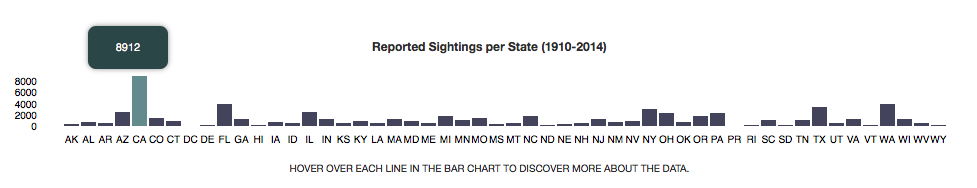
\includegraphics[width=\textwidth]{sightings_count.png}
%\label{sightings}
%\end{figure*}
%
%\begin{figure*}
%\centering
%\caption{Interactive national map of sightings with year slider bar and brushable chart of durations and donut chart of shapes of sightings. Mouse is hovering over a sighting in North Dakota and tooltip is displaying }
%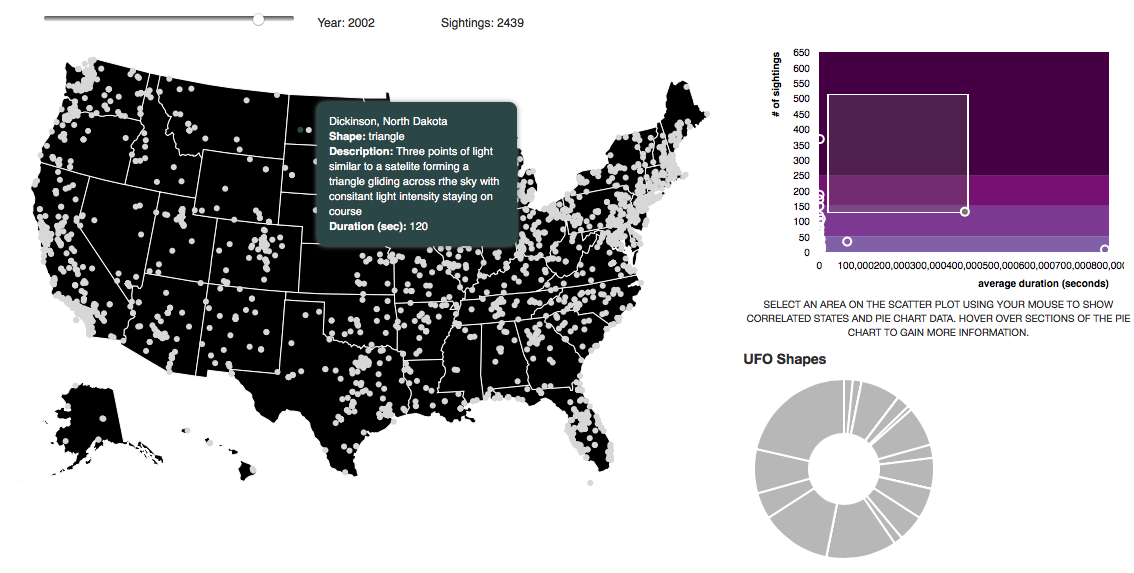
\includegraphics[width=\textwidth,height=8cm]{map.png}
%\label{map}
%\end{figure*}

%\begin{figure}
%\centering
%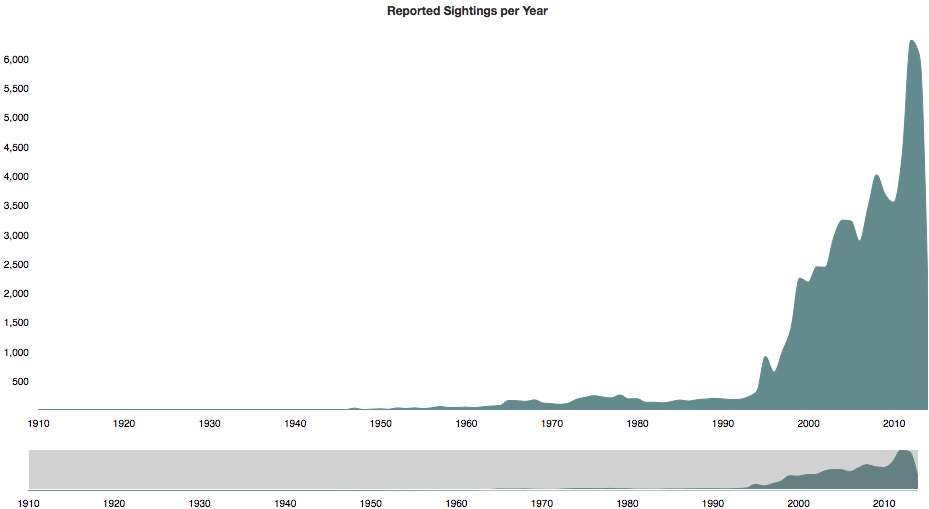
\includegraphics[width=3.4in]{timeline.png}
%\caption{Interactive timeline of UFO sightings from 1910-2014}
%\label{timeline}
%\end{figure}








%In general these tasks can be categorized into two abstract tasks.
%\begin{itemize}
%\item \textbf{(T1)} Overview task:
%\item \textbf{(T2)} Drill-Down task:
%\end{itemize}



\section{Design}
%For the abstract tasks, we chose the following visualization idioms (Table 3).


%\begin{table}[h]
%\caption{Visualizing the Abstract Tasks} % title name of the table
%\centering % centering table
%\begin{tabular}{c c c} % creating 3 columns
%\hline\hline % inserting double-line
% Abstract Task & Visualization Idiom\\ [0.5ex]
%\hline % inserts single-line
%
%Overview & Map\\[1ex] %space
%
%Drill-Down & Map and Line Chart\\[1ex] %space
%
%\hline 
%\end{tabular}
%\label{tab:PPer}
%\end{table}

%\textbf{Visual Encoding and Interaction Choices:}
%
%\begin{itemize}
%
%\item Points on map for representation of geographic data
%\item Sequential color scale for frequency of sightings on choropleth map
%\item Retrieve details of sighting on tooltip on hover
%\item Clicking on state to change the drilled-down view (hovering only affects tooltip)
%\item Line chart for frequency of sightings of state over time (position as a channel for quantitative value)
%\item Brush to choose sightings of an area for which the user wants to know information about when they occurred
%
%\end{itemize}


Our final visualization shows the data in many different ways, all including interactivity to different degrees, which allows the user to decide which path through the story they want to take. When they first load the page, the user greeted by a clean layout, banner, and explanatory text. This serves to make the page seem inviting and encourage the user to read the motivation and explore the tools. Our first visualization is intentionally visible without scrolling, which shows the number of reporting sightings over the history of our data set; this is the highest level of data encoded. The user can hover the mouse over a bar and see a tool tip display the number of sightings in that state in total from 1910-2014.

\begin{figure}[h]
\centering
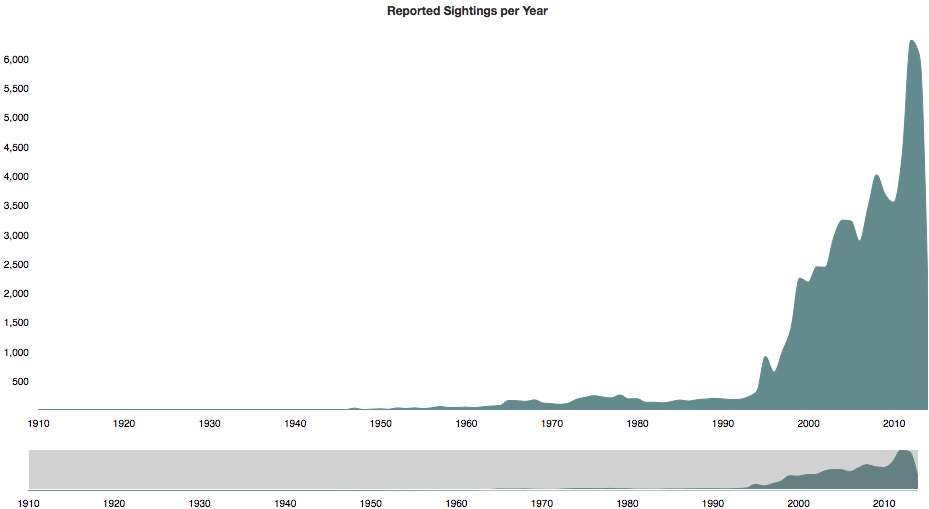
\includegraphics[width=3.4in]{timeline.png}
\caption{Interactive timeline of UFO sightings from 1910-2014}
\label{timeline}
\end{figure}


After reading what is immediately visible, the user will notice that there is more material cut off at the bottom of the screen. This will lead the user to discover our next interactive feature. The next visualization (Figure \ref{timeline}) shows the reporting sightings per year and allows the user to zoom in and brush the data that they are interested in seeing; there are two ways to brush down the data; on the time series and on the chart itself. If a user is scrolling down the page, they will likely inadvertently discover that scrolling the mouse while the cursor is hovering over the time series chart will cause it to zoom in. This is intended to peak curiosity and allow the user to realize that all the visualizations have an interactive features.

\begin{figure*}[h]
\centering
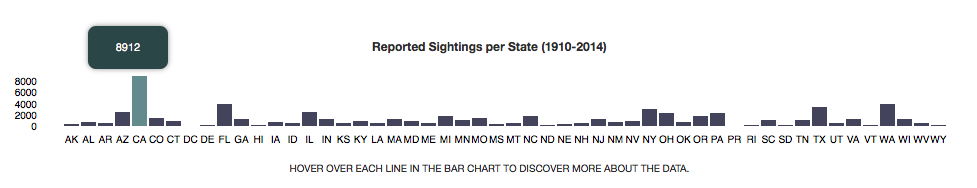
\includegraphics[width=\textwidth]{sightings_count.png}
\caption{Interactive bar graph of the total number of sightings by state, with mouse hovering over California}
\label{sightings}
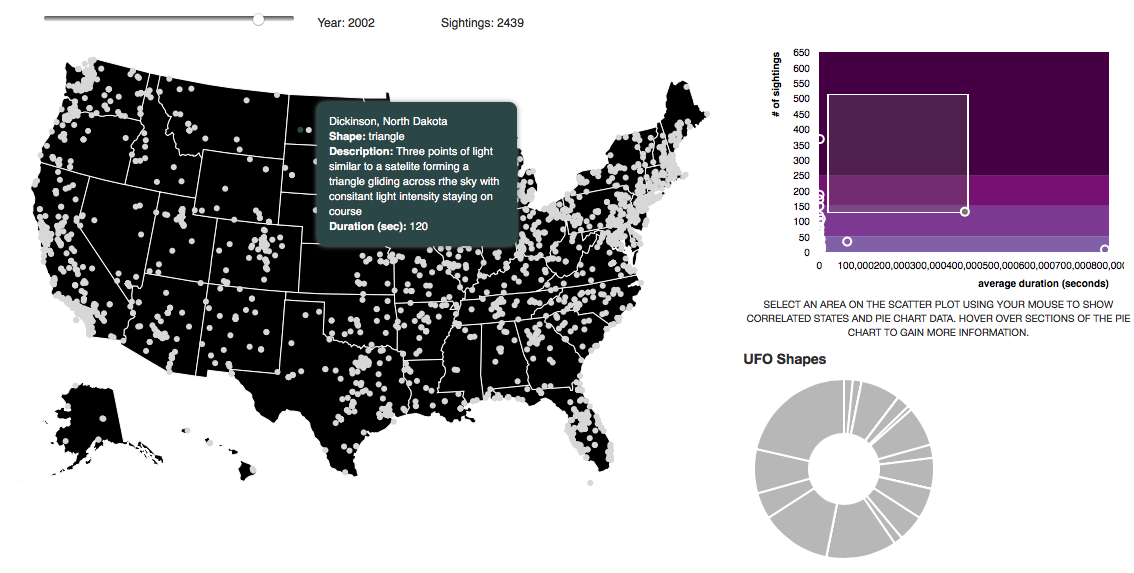
\includegraphics[width=\textwidth]{map.png}
\caption{Interactive national map of sightings with year slider bar and brushable chart of durations and donut chart of shapes of sightings. Mouse is hovering over a sighting in North Dakota and tooltip is displaying }
\label{map}
\end{figure*}


Our final visualization (Figure \ref{map}) appears shortly after a little more text, showing the geo-location of each individual sighting during the selected year. The user selects the year using the slider above the map, which populates using points in the exact geo-location for that specific year. The total number of sightings for that year is also displayed on top of the map and the map has an on-click feature, which allows the user to drill down to a state level for more specific information with the data points and ease of access in using the tool tip. The choropleth map is color coded by the number of sightings in a particular state. The shade of purple displayed is the same as the shade in the scatterplot to the right, which allows the scatterplot to serve as a legend for the color. That scatter plot displays points that indicate states, and the axes reflect the number of sightings versus average duration. The donut plot shows the proportion of shapes sighted, either by year on a national level, using the brushed data from the scatter plot. A user can also hover over the donut plot to see what shape is represented, as is demonstrated by the tooltip in Figure \ref{map}.

This visualization was built using HTML, CSS, JavaScript, and several open-source projects including D3 v4, d3-queue, Moment JS, jQuery, topojson, Underscore JS, Bootstrap, and NodeJs. \footnote{\url{https://emily-jean.github.io}}

\section{Discussion}
\subsection{Reflection}
The main purpose of this project is to serve as a way to explore the data hosted on the National UFO Report Center's website. The data set hosted there is massive and hard to understand without performing analysis, so any visual representation of the data would be useful to someone interested. Fortunately, the data was extremely well formatted and easy to access and work with. The related work with this data could also be improved with further interactivity and so this project seemed a good fit for our class. Now that it is complete it is clear that this visualization was an improvement on the existing ones that work with this data set. 

An effective method we used to pick our design was study the related work for features that we liked and features we would have liked that were missing. We immediately liked the use of a map and overlaying of the spacial data of the sightings, but due to the large number of points, we were able to know from the beginning that we wanted to incorporate a feature that lets a user zoom in on the map and see sightings over a smaller area. We also decided that the slider at the top to view sightings by year would simplify the data as well, and reflecting on the finished product seems to confirm that it was a good decision. 

Looking back at all the initial design sketches, they were overall useful to have done as iterations. We had more than twelve initial design sketches to work off of, and none were constrained by implementation limitations or the actual data. Some of the initial design sketches had a separate window appearing when you clicked on a state, and would display sightings across all years from 1910-2014 on that state. It turned out that it was easy to underestimate the volume of data we would be representing. Combining all the sketches forced us to focus on what limitations we might encounter when implementing an idea. Therefore, we found that creating a single work flow to work towards was valuable in the design phase. It forced all of us to agree upon a single design and make that design more representative of what would be feasible to create in a limited time frame. 

Usability testing was the last milestone before completing development of our visualization. We had classmates from our visualization class test our prototype and studied how they approached the tool as well as solicited feedback from the subjects. This visualization is geared towards users interested in exploring the data, so there is no particular ideal test user. Because of this, we were able to get impactful and varietal feedback during user testing. We decided to include more explicit instructions to users on the website that they could click on the map to zoom in and brush points in the lower scatter plot and see the correlated states and pie chart data showing the shapes of the sightings. Without explicit instructions, some users didn't know these features existed or would only discover them after a long time. Since the user testing phase was very easy to conduct, we found the whole process well worth doing and overall helpful.


\subsection{Future Work}
This paper focused on the UFO data we worked with, the tasks we sought to implement, and the visualization design that resulted from these requirements as well as through acquired feedback. There are many features we would like to be able to include in the future. Among the most interesting would be to associate historical weather data with the dates of the alleged UFO sightings. Additionally, plotting sources of red flags such as airports or weather balloons would be of use in explaining a large number of sightings. The biggest challenge at the moment is acquiring a suitable data set containing this information in a reasonable format. 


\section{Conclusion}
We created a web-based interactive visualization providing a novel view of data originally gathered by the National UFO Report Center of thousands of alleged UFO sightings around the country. We incorporated interactivity tools such as brushing and linking to make it easier to dynamically view reported sightings on a United States map and select only reports within years ranges of interest. This allows a map to be less cluttered than existing maps and thus also allows for details-on-demand to be easier to use as there is less ambiguity of where a user is pointing. We use an appealing color palate for the task at hand and create an environment that is amusing and engaging to users interested in understanding the scale of belief in conspiracies or UFOs.




\begin{thebibliography}{9}

\bibitem{blocks} 
Mike Bostock.
\textit{Blocks}. 
Click-to-Zoom via Transform,
\\\url{https://bl.ocks.org/mbostock/2206590}

\bibitem{ufoimage} 
Newsweek.
\textit{UFO existence proven beyond reasonable doubt says former head of Pentagon alien program}.
\\\url{http://www.newsweek.com/ufo-existence-proven-beyond\\-reasonable-doubt-says-former-head-pentagon-alien-758293}

\bibitem{dataduo}
DataDuo - DuoDare Project on UFO sightings
\\\url{https://thedataduo.com/2017/11/11/duodare-3\\-ufo-sightings/}

\bibitem{ufowiki}
Wikipedia.
\textit{Unidentified flying object}.
\\\url{https://wikipedia.org/wiki/Unidentified\_flying\_object}

\bibitem{history}
History.
\textit{History of UFOs}.
\\\url{https://www.history.com/topics/history-of-ufos}

\bibitem{pentagon}
The Guardian.
\textit{Pentagon admits running secret UFO investigation for five years}.
\\\url{https://www.theguardian.com/world/2017/dec/17/\\pentagon-admits-running-secret-ufo-investigation-for-five-years}

\bibitem{listen}
The Guardian.
\textit{Why we keep scanning the skies for signs of alien intelligence}.
\\\url{https://www.theguardian.com/science/2017/dec/22/\\why-we-keep-scanning-the-skies-for-signs-of-alien-intelligence}

\bibitem{listenwiki}
Wikipedia.
\textit{Breakthrough Listen}.
\\\url{https://en.wikipedia.org/wiki/Breakthrough\_Listen}

\bibitem{hawking}
Newsweek.
\textit{Stephen Hawking on alien life, extraterrestrials and the possibility of UFOs visiting Earth}.
\\\url{http://www.newsweek.com/stephen-hawking-death-alien\\-contact-aliens-theory-ufo-search-breakthrough-844920}

\bibitem{projections}
Geokov.
\textit{Map Projections - Types and Distortion Patterns}
\\\url{http://geokov.com/education/map-projection.aspx}

\bibitem{distortion}
Mike Bostock.
Map Projection Distortions
\\\url{https://bl.ocks.org/mbostock/3709000}

\end{thebibliography}





%% if specified like this the section will be committed in review mode


%\bibliographystyle{abbrv}
\bibliographystyle{abbrv-doi}
%\bibliographystyle{abbrv-doi-narrow}
%\bibliographystyle{abbrv-doi-hyperref}
%\bibliographystyle{abbrv-doi-hyperref-narrow}

\bibliography{template}
\end{document}

